We apply the two Network Guided Estimators to factor model residual covariance matrix. Assume that the excess returns have the following factor structure
\begin{equation*}
    Y_{it} = B_{i}'F_{t} + \epsilon_{it}
\end{equation*}
and we assume that \(\Sigma = [E \epsilon_{i} \epsilon_{j}]_{1 \leq i,j\leq N}\) is sparse.

We collect daily return data on SP500 stock from 2004 to 2015 from CRSP, together with daily data on Fama-French 3 factors and the risk free rate.  We do a rolling window analysis, each window consists of an estimation period of 252 days and a testing period of 21 days. In the estimation period, we estimate the factor loadings by linear time series regression of excess return \(Y_{it}\) on \(F_{t}\), hence allowing the betas to vary over time, and find the de-factored excess return by 
\begin{equation*}
    \hat{\epsilon}_{it} = Y_{it} - \hat{B}_{i}'F_{t},
\end{equation*}
and we estimate \(\Sigma_{\epsilon}\) by the Network Guided Estimator applied to \(\hat{\Sigma}_{\epsilon} = \frac{1}{T} \sum_{t}\hat{\epsilon}_{t} \hat{\epsilon}_{t}'\).


We now introduce the auxiliary network information that we use. The first network we have is the \textit{News-Implied Network}. The news data are obtained from RavenPack Equity files Dow Jones Edition for the period January 2004 to December 2015. This comprehensive news dataset combines relevant content from multiple sources, including Dow Jones Newswires, Wall Street Journal, and Barron's MarketWatch, which produce the most actively monitored streams of news articles in the financial system. Each unique news story (identified by a unique story ID) tags the companies mentioned in the news by their unique and permanent entity identifier codes (RP\_ENTITY\_ID),  by which we link to stock identifier TICKER and PERMNO. Same as \cite{ge2022news}, we identify links by news co-mentioning. That is, if a piece of business news reports two companies together, they share a link. We do not consider the news that co-mention more than two companies since although they may carry potential information about links, they provide noisier information. We also remove news with topics including analyst recommendations, rating changes, and index movements, as these types of news might stack multiple companies together when they actually do not have real links. \autoref{table:news} and \autoref{table:freq} in Apprendix provide descriptive statistics for RavenPack Equity files Dow Jones Edition dataset during the sample period. Since our comprehensive news dataset combines several sources, given a similar length of sample period, the number of unique news stories is more than ten times larger than that from \cite{scherbina2015economic} and more than eight hundred times than that from \cite{schwenkler2019network}. For link identification purposes, we only use sample news (1) are not about topics mentioned above, (2) tag $S\& P$ $500$ companies and (3) mention exactly two companies, which is a subsample of $1,637,256$ unique news stories. The second network we consider is the \textit{Analyst Coverage Network}.  It has been documented that shared analyst coverage is a strong proxy for fundamental linkages between firms and reflects firm similarities along many dimensions (\cite{ali2020shared}, \citet{israelsen2016does}, \citet{kaustia2013common}). We use the Institutional Brokers Estimate System (IBES) detail history files to construct the analyst co-coverage-based adjacency matrix. For each year in the sample, we consider a stock is covered by an analyst if the analyst issues at least one FY1 or FY2 earnings forecast for the stock during the year. And we consider two stocks as linked if there are common analysts during the year, weighted by the number of common analysts. We then add up the yearly adjacency matrices to get the full sample adjacency matrix.  We also consider a couple of \textit{Industry-Based Networks}. This is motivated by \cite{moskowitz1999industries}, \citet{engelberg2018know} that stocks within the same industry exhibit excess co-movement.  Utilizing this fact in the estimation of large covariance matrices, \cite{fan2016incorporating} apply location-based thresholding based on GICS sector classification. We consider industry classification based on The Standard Industrial Classification (SIC). In particular, we consider two stocks to be linked if they have the same 4-digit (3-digit) SICCD code, and thus we have two block-diagonal network matrices where companies within the same industry are fully connected. Lastly, we consider a \textit{Customer-Supplier Network} (\cite{cohen2008economic}). The links are obtained from Andrea Frazzini's data library, where strength of links is weighted by sales.

To demonstrate the usefulness of auxiliary network information in capturing pairs with non-zero correlations, we plot the histograms of factor model residual correlations for all non-diagonal elements (all possible pairs among entities) and only the linked pairs (implied by the aforementioned auxiliary network information). \autoref{fig:corr5factors} show the histograms of Fama-French 5-factor model residual correlations. From the top left plot, we find that after removing five FF factors, the remaining correlations are mostly zero or take small values around zero. In contrast, the correlation distributions are positively skewed among linked pairs, 
and the probability of having zero correlation is much lower. Taking the upper right plot as an example, most of the stock pairs that are co-covered by analysts have positive residual correlations, and the number of pairs having zero correlation is very small (i.e., type I error is small). This indicates that our auxiliary network information is useful in identifying the pairs with non-zero correlations. In \autoref{fig:corr5factors} of the Appendix, we plot the histograms of residual correlations after removing five principal components, and similar patterns are found.
\begin{figure}[H]
    \centering
    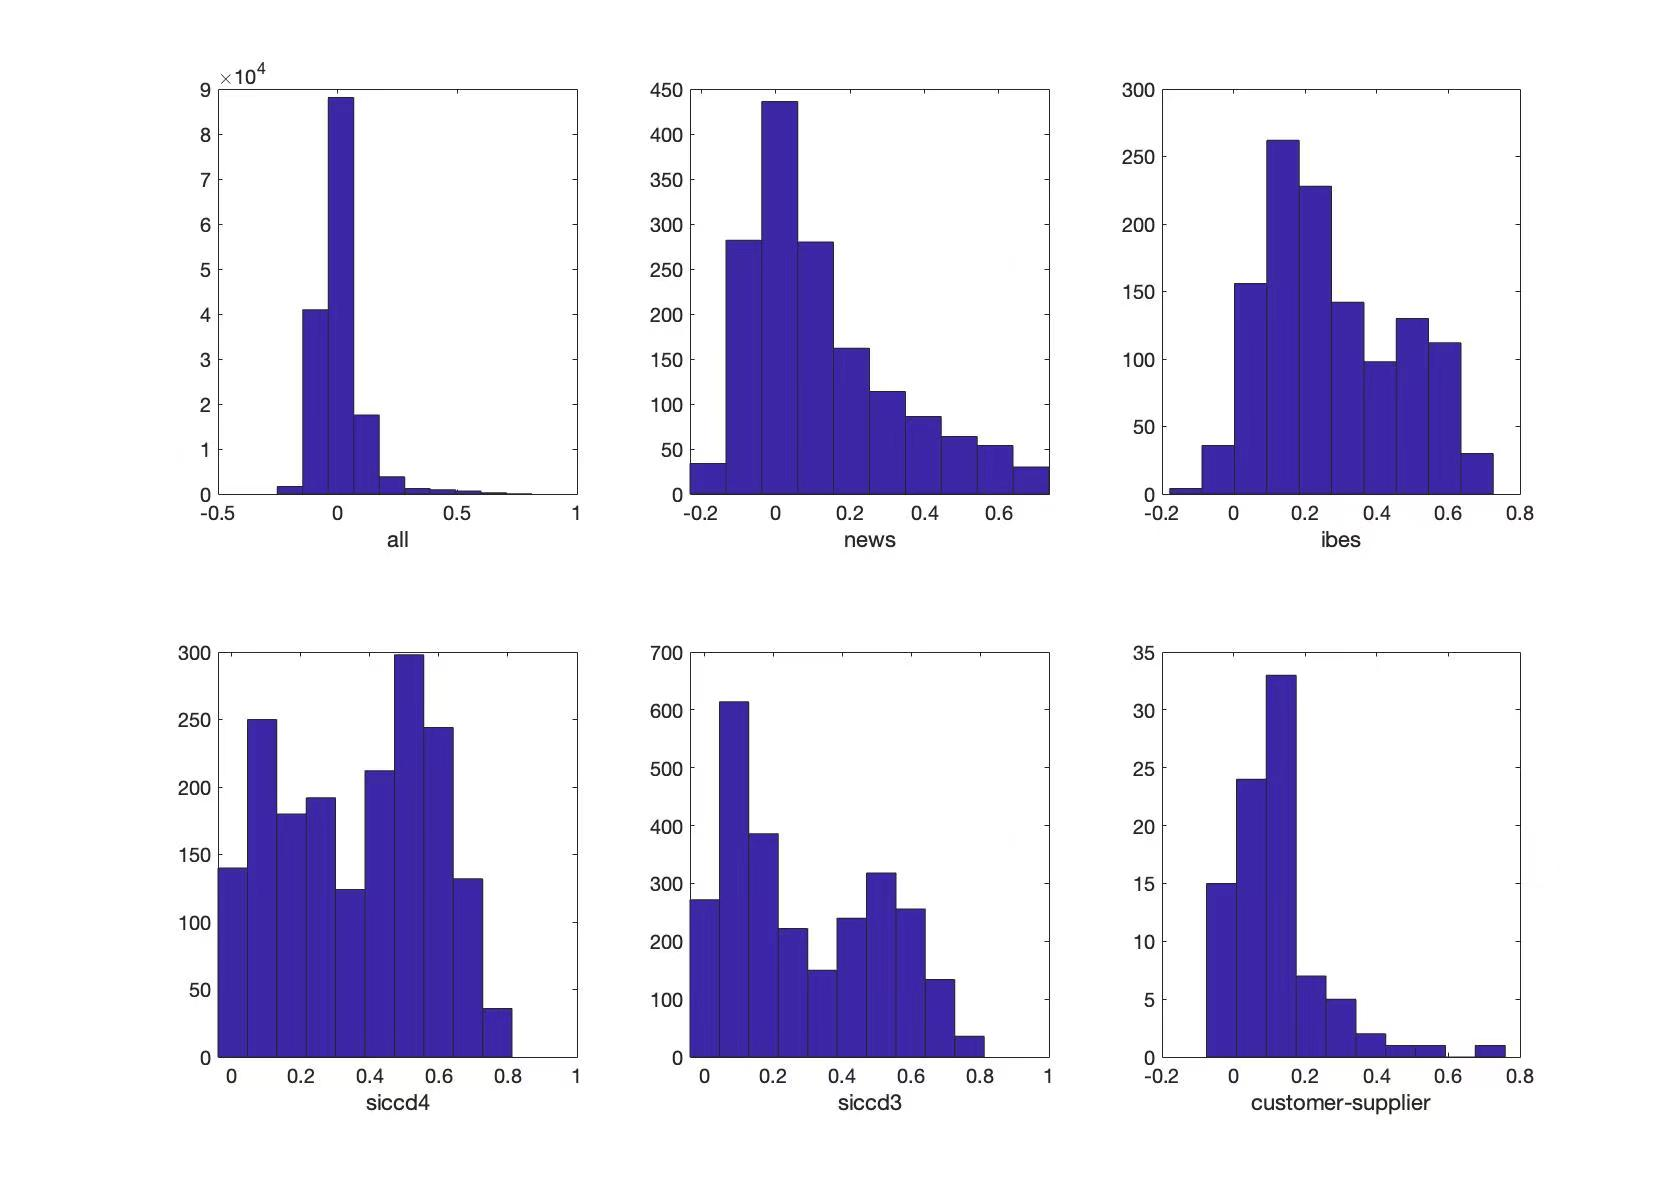
\includegraphics[scale=0.25]{pic/corr_5factors.jpg}
    \caption{Histograms of factor model residual correlations. Correlations are calculated on the Fama-French 5-factor model residuals. The top left sub-figure shows the histogram of all non-diagonal residual correlations. The rest sub-figures show the histograms of residual correlations among linked pairs.}
    \label{fig:corr5factors}
\end{figure}

Next, we apply the proposed method to a portfolio management problem. In particular, we consider the estimation of Global Minimum Variance (GVM) portfolio as in \cite{ledoit2004HoneyShrunk}. The key is to estimate the covariance matrix of asset returns (i.e.,$\Sigma_{Y}$) as weight of such portfolio is given by
\begin{equation*}
    w = \frac{\Sigma_{Y} \mathbf{1}}{\mathbf{1}' \Sigma_{Y} \mathbf{1}},
\end{equation*}
where \(\mathbf{1}\) is a conforming vector of ones. Given the factor structure,  we have
\begin{equation*}
    \Sigma_{Y} = B \Sigma_{F} B' + \Sigma_{\epsilon}
\end{equation*}
We do a rolling window analysis, where each window consists of an estimation period of 252 days and a testing period of 21 days. In the estimation period, we first estimate the factor model, and then apply Network Guided Estimator to the factor model residual covariance matrix. Having \(\hat{B} ,\hat{\Sigma}_{F}, \hat{\Sigma}_{\epsilon}\), we then construct $\hat{\Sigma}_{Y} = \hat{B} \hat{\Sigma}_{F} \hat{B}' + \hat{\Sigma}_{\epsilon}$ and derive the \textit{global minimum variance} portfolio where weights are $w = \frac{\hat{\Sigma}_{Y} \mathbf{1}}{\mathbf{1}' \hat{\Sigma}_{Y} \mathbf{1}}$.  We collect the portfolio return over the next 21-day testing period. This constitutes one of the rolling windows. Then we move forward 21 days and repeat this exercise. Using 2004- 2014 daily data, we can construct a daily portfolio return from 2005 to 2015, where the portfolio is re-balanced every 21 days. We compute the holding period return of this portfolio and its standard deviation. The results are summarized in \autoref{table:GVP}. 
\begin{table}[H]
    \centering
    \begin{tabular}{lr}
\toprule
Estimator &  Out-of-sample standard deviation of GMV portfolio              \\
\midrule
Network Guided Thresholding      &              0.0255  \\
Linear Shrinkage       &               0.0264\\
Universal Thresholding &                0.0263  \\
Equally Weighted        &        0.0667\\
\bottomrule
\end{tabular}
    \caption{Out-of-sample performance of each method}
    \label{table:GVP}
\end{table}
As discussed in \cite{engle2019large} and \cite{chen2019new}, 
to judge the performance of a covariance matrix estimation method by the global minimum variance (GMV) portfolio, the most important measure is the constructed portfolio's out-of-sample volatility. In this respect, the global minimum variance portfolio constructed using the covariance matrix estimated using \textit{Network Guided Thresholding} has the smallest out-of-sample standard deviation.  Notice that the empirical results are preliminary, and we are still figuring out how to utilize those auxiliary better information. 
